\documentclass{article}
\usepackage[utf8]{inputenc}
\usepackage{longtable}
\usepackage{gensymb}
\usepackage{graphicx}
\usepackage{siunitx}
\usepackage{caption}
\usepackage[colorlinks,bookmarks=false,citecolor=blue,linkcolor=blue,urlcolor=blue]{hyperref}
\usepackage{relsize}
\usepackage{amsmath}
\usepackage{amssymb}
\usepackage{bm}
\usepackage{multirow}

\begin{document}
\begin{titlepage}
\begin{center}

\includegraphics[scale=0.12]{document/niser.png}
\line(1,0){340}\\
[2mm]
\begin{large}
\textbf{\huge The Fabry-Perot Interferometer}\\ 
\end{large}
\line(1,0){200}\\
[5cm]
\large MAITREY SHARMA\\
\small (1911093)\\
[3.5cm]
Third Year Integrated M.Sc.\\
\textbf{School of Physical Sciences}\\
\textbf{National Institute of Science Education and Research, Bhubaneshwar}\\
\small August 31, 2021
\end{center} 
\end{titlepage}
\newpage
\section{Aim}
\begin{itemize}
    \item Alignment of Fabry-Perot Interferometer to observe concentric circular fringes.
    \item Measurement of the wavelength of a diode Laser.
    \item Determination of difference in wavelengths of sodium doublet.
\end{itemize}
\section{Apparatus}
\begin{enumerate}
    \item Optical Rail (1 meter),
    \item Fabry-Perot setup (Fixed Mirror mount with Two Etalon),
    \item Movable Mirror with Kinematic and fine linear Micrometer (0-10 mm),
    \item Diode Laser mount with Kinematic (5 V) Power Supply,
    \item Achromatic Lens mount,
    \item Frosted Glass viewing Screen and mount with Micrometer.
\end{enumerate}

\section{Introduction}
\noindent The Fabry–Perot interferometer is based on the principle of \textbf{multiple-beam interferometry}. The interferometer (as shown in figure (\ref{fig:etalon})) consists of two plane glass (or quartz) plates which are coated on one side with a partially reflecting metallic film (of aluminum or silver) of about $80\%$ reflectivity. These two plates are kept in such a way that they enclose a plane parallel slab of air between their coated surfaces. If the reflecting glass plates are held parallel to each other at a fixed separation, we have a \textit{Fabry–Perot etalon}. 
\begin{figure}[h!]
    \centering
    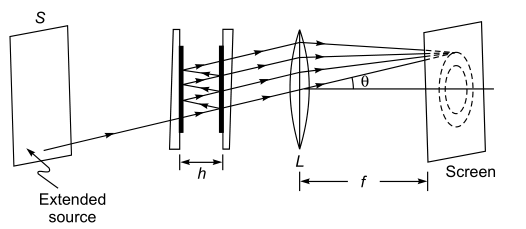
\includegraphics[scale = 0.85]{Figures/fabry perot etalon.png}
    \caption{The Fabry-Perot Etalon}
    \label{fig:etalon}
\end{figure}
\par
\noindent
If one of the mirrors is kept fixed while the other is capable of moving to change the separation between the two mirrors, the system is called a \textbf{Fabry–Perot interferometer}. Each time the light encounters one of the surfaces, a portion of it is transmitted out, and the remaining part is reflected back. The net effect is to break a single beam into multiple beams which interfere with each other. If the additional optical path length of the reflected beam (due to multiple reflections) is an integral multiple of the light's wavelength, then the reflected beams will interfere constructively. More is the number of reflection inside the cavity, sharper is the interference maximum. The Fabry-Perot interferometer can be used as a spectroscopic tool to understand concepts of finesse (a coefficient which describes the reflectivity of the mirrors in the interferometer)and free spectral range (the spacing in optical frequency or wavelength between two successive reflected or transmitted optical intensity maxima or minima of an interferometer).

\section{Construction}
\noindent
Two partial mirrors $G_1$ and $G_2$ are aligned parallel to one another at a distance $d$, forming a reflective cavity. When irradiated by a monochromatic light (a laser here) of wavelength $\lambda$ at an angle of incidence $\theta$, multiple reflections takes place inside the cavity (see figure (\ref{fig:schematics})).

\begin{figure}[h!]
    \centering
    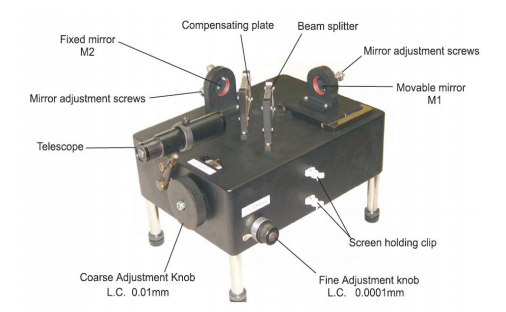
\includegraphics{Figures/schematics.png}
    \caption{Schematics of a Fabry-Perot interferometer}
    \label{fig:schematics}
\end{figure}
\par
\noindent
Part of the light is transmitted each time the light reaches the second reflecting surface. All such transmitted light rays interfere with each other to give rise to a maxima or minima depending on the path difference between them.


\section{Theory}
\noindent Let $n$ be the refractive index of the medium in the cavity (in this case it is air), Then the optical path difference between two neighboring rays is
\begin{equation}
    \label{eq1}
    \Delta = 2 n d \cos \theta
\end{equation}
Then the phase difference, $\delta$ is given by
\begin{equation}
    \delta = \frac{2 \pi}{\lambda} \Delta
\end{equation}

\begin{figure}[h!]
    \centering
    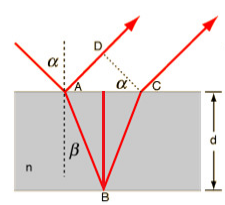
\includegraphics[scale = 0.8]{Figures/calc of path diff.png}
    \caption{Calculation of path difference}
    \label{fig:pathdiff}
\end{figure}
\noindent
From the figure (\ref{fig:pathdiff}) we have,
\begin{equation}
    \Delta = n (AB + BC) - AD;
\end{equation}
\begin{equation}
    AB = \dfrac{d}{\cos \beta};
\end{equation}
\begin{equation}
    AD = (2 d \tan \beta) \sin \alpha
\end{equation}
\noindent
Using Snell's law, 
\begin{equation}
    AD = 2d \tan \beta (n \sin \beta)
\end{equation}
\begin{equation}
    \implies \Delta = 2 n d \Bigg[\dfrac{1}{\cos \beta} - \tan \beta \sin \beta \Bigg]
\end{equation}
\begin{equation}
    \implies \Delta = 2 n d \Bigg[\dfrac{1 - \sin^2 \beta}{\cos \beta} \Bigg] = 2 n d \cos \beta
\end{equation}
\noindent
Thus, the resultant light intensity $I_T$ is given by
\begin{equation}
    I_T = I_0 \dfrac{1}{1 + \Bigg[ \dfrac{4R}{(1 - R)^2} \sin^2 \bigg(\dfrac{\delta}{2}\bigg) \Bigg]}
\end{equation}
\noindent
where $I_0$ is the incident intensity and $R$ is the reflectivity of the mirrors. It can be noted that $I_T$ varies with $\delta$ and we can conclude that,
\begin{center}
    $\Delta = m \lambda$ or $\delta = 2 m \pi$ \hspace{1cm} (for maxima, $m \in \mathbb{N}_0$)\\
    $\Delta = (2 m + 1) \lambda / 2$ or $\delta = (2 m + 1) \pi$ \hspace{0.3cm} (for minima, $m \in \mathbb{N}_0$)
\end{center}
\noindent
The complete interference pattern appears as a set of concentric rings (see figure (\ref{fig:cgrings})). 
\begin{figure}[h!]
    \centering
    \captionsetup{justification=centering}
    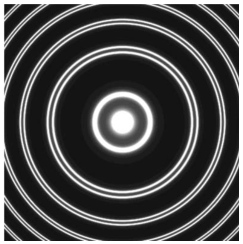
\includegraphics[scale = 1]{Figures/cgrings.png}
    \caption{The (computer generated) ring pattern as obtained (on the focal plane of a lens) in a Fabry–Perot etalon}
    \label{fig:cgrings}
\end{figure}
\par
\noindent
The sharpness of the rings depends on a parameter called coefficient of finesse, $F$, defined as
\begin{equation}
    F = \dfrac{4R}{(1 - R)^2}
\end{equation}
\noindent
We can use the relations obtained above to determine the wavelength of incident light, $\lambda$ accurately. Let the initial separation between the mirrors is $d_1$. If one counts the number of fringes (say maxima) appearing or disappearing at the centre ($\theta \approx 0$) by varying the distance between the mirrors to $d_2$, then $\lambda$ can be determined as follows:
\begin{center}
    $2 d_1 = m_1 \lambda$\\
    $2 d_2 = m_2 \lambda$
\end{center}
If $(m_2 - m_1)$ is the number of maxima counted, we have
\begin{equation}
    \boxed{\lambda = \dfrac{2 (d_2 - d_1)}{m_2 - m_1}}
\end{equation}
\par
\noindent
The Fabry-Perot interferometer can be used for measurement of the wavelength separation of sodium 
D-lines which lie are very close to each other, i.e. \SI{588.9950}{\nano \metre}  and \SI{589.5924}{\nano \metre}. Therefore, during the process of moving the interferometer's movable mirror, the interference fringes produced by the two yellow lines will appear periodically clear and blurry (due to splitting). For a given separation ($2 d_1$) of the mirrors, maxima of the two wavelengths coincide to give a clear fringe pattern and satisfy the following relation:
\begin{center}
    $2 d_1 = m_1 \lambda$\\
    $2 d_2 = m_2 \lambda$
\end{center}
\noindent
where $m_1$ and $m_2$ are respective orders of maxima for $\lambda_1$ and $\lambda_2$. Due to difference in wavelength, when the mirror is moved the corresponding fringes will not move equally and 
the pattern will be blurry. On further movement the pattern becomes clear again where the $m$th order of the longer wavelength coincides with $(m + 1)$th order of the shorter wavelength. 
Assuming $\lambda_1 > \lambda_2$, we can write the above obtained relation as
\begin{equation}
    2 (d_1 + d) = m_1 \lambda_1 = (m_1 + 1) \lambda_2
\end{equation}
\par
\noindent
If $\lambda$ is the average of $\lambda_1$ and $\lambda_2$ (so that $\lambda_1 \lambda_2$ can be approximated as $\lambda^2$), then the difference of two wavelengths, $\Delta \lambda$, can be represented as
\begin{equation}
\label{eq13}
    \boxed{\Delta = \dfrac{\lambda^2}{2 d}}
\end{equation}
\par
\noindent
For a beam incident normally on the interferometer, we vary the separation h and measure the intensity variation on the focal plane of lens $L$ as shown in figure (\ref{fig:scanning}). Such an arrangement is usually referred to as a scanning Fabry–Perot interferometer.
\begin{figure}[h!]
    \centering
    \captionsetup{justification=centering}
    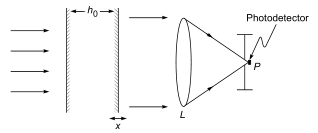
\includegraphics{Figures/scanning.png}
    \caption{A scanning Fabry–Perot interferometer. The intensity variation is recorded (by a photo-detector) on the focal plane of lens $L$.}
    \label{fig:scanning}
\end{figure}
\clearpage
\section{Experimental Setup}
\begin{figure}[h!]
    \centering
    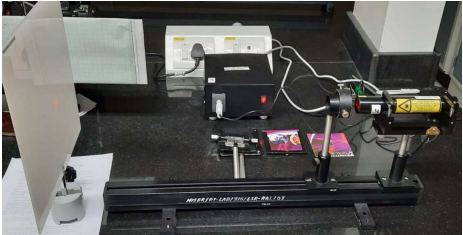
\includegraphics[scale = 0.65]{Figures/setup.png}
    \caption{Setup with Laser as the source}
    \label{fig:setup}
\end{figure}
\begin{figure}[h!]
    \centering
    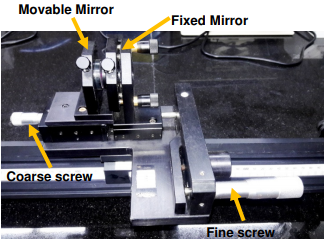
\includegraphics[scale = 1]{Figures/interfero.png}
    \caption{Setup with Na lamp as source}
    \label{fig:interfero}
\end{figure}


\section{Observations}
\begin{enumerate}
    \item Least count of fine micrometer = \SI{0.01}{\milli\metre}
    \item Initial position of fine micrometer, $d_1 = \SI{24}{\milli \metre}$
    \item Lever ratio, $r = 0.03$.
\end{enumerate}
\begin{table}[h!]
\centering
\caption{\textbf{Data for Diode Laser}}
\begin{tabular}{ccccccc}
\hline
\hline
\textbf{\#} & \begin{tabular}[c]{@{}c@{}} \textbf{No. of} \\ \textbf{fringes} \\ \textbf{appeared} \\ \boldmath $ (m_2 - m_1)$ \end{tabular} & \begin{tabular}[c]{@{}c@{}} \textbf{Main} \\ \textbf{scale} \\ \textbf{reading},\\ (mm) \end{tabular} & \begin{tabular}[c]{@{}c@{}} \textbf{No. of} \\ \textbf{divisions} \\ \textbf{rotated} \end{tabular} & \begin{tabular}[c]{@{}c@{}} \boldmath $d_2$ \\ (mm) \end{tabular} & \begin{tabular}[c]{@{}c@{}} \boldmath $\Delta d$ \\ \boldmath $|d_2 - d_1|$ \\ (mm)\end{tabular} & \begin{tabular}[c]{@{}c@{}} \textbf{Actual} \\ \textbf{distance} \\ \textbf{moved} \\ (mm)\end{tabular} \\ \hline \hline
1      & 10                                                           & 23.5                                                                              & 38                                                                           & 23.88                                            & 0.12             & 0.0036                                 \\ 
2      & 20                                                           & 23.5                                                                              & 26                                                                            & 23.76                                            & 0.24            & 0.0072                                  \\ 
3      & 30                                                           & 23.5                                                                              & 14                                                                           & 23.64                                            & 0.36            & 0.0108                                  \\ 
4      & 40                                                           & 23.5                                                                              & 2                                                                           & 23.52                                            & 0.48            & 0.0144                                  \\ 
5      & 50                                                           & 23                                                                              & 41                                                                            & 23.41                                            & 0.59            & 0.0177                                 \\ 
6      & 60                                                           & 23                                                                              & 29                                                                           & 23.29                                            & 0.71            & 0.0213                                  \\ 
7      & 70                                                           & 23                                                                              & 17                                                                           & 23.17                                            & 0.83            & 0.0249                                 \\ 
8      & 80                                                           & 23                                                                              & 7                                                                           & 23.07                                            & 0.93            & 0.0279                                 \\ 
9      & 90                                                           & 22.5                                                                              & 45                                                                           & 22.95                                            & 1.05            & 0.0315                                 \\
10     & 100                                                          & 22.5                                                                              & 35                                                                           & 22.85                                            & 1.15            & 0.0345                                 \\ \hline
\hline
\end{tabular}
\label{Tab:diodeLaser}
\end{table}

\begin{table}[h!]
\centering
\caption{\textbf{Data for Na Lamp \\ $\Delta \lambda = \lambda / 2 ( \Delta d)^2$}; $\lambda = \SI{589}{\nano \metre}$}
\begin{tabular}{cccr}
\hline
\hline
\textbf{\#} & \boldmath $\Delta d$ (mm)  & \boldmath $\Delta \lambda$ (nm) & \multicolumn{1}{c}{\boldmath $<\Delta \lambda>$}  \\ \hline
\hline
1      & 0.2511 & 0.6908  & \multirow{5}{*}{0.6822} \\
2      & 0.2520 & 0.6883  &                              \\
3      & 0.2574 & 0.6739  &                              \\
4      & 0.2475 & 0.7009  &                              \\
5      & 0.2640 & 0.6570  &                              \\ \hline
\hline
\end{tabular}
\label{Tab:NaLamp}
\end{table}

\section{Graphs}
\begin{figure}[h!]
    \centering
    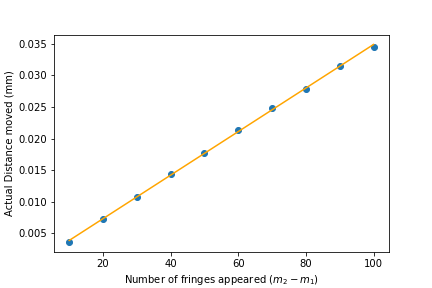
\includegraphics[scale = 0.5]{Figures/plot.png}
    \caption{Actual distance moved vs $(m_2-m_1)$ plot for the Diode Laser}
    \label{fig:laserplot}
\end{figure}

\section{Calculations}
    We first analyse the plot (figure~(\ref{fig:laserplot})) obtained from the table~(\ref{Tab:diodeLaser}).
    The five summations for this data-set are as follows:
    \par
    \vspace{0.5cm}
    $S_{x} = \mathlarger{\mathlarger{\sum}} x_{i} = 550$, \hspace{1cm} $S_{y} = \mathlarger{\mathlarger{\sum}} y_{i} = \SI{0.1938}{\milli \metre}$,
    \par
    \vspace{0.5cm}
    $S_{xx} = \mathlarger{\mathlarger{\sum}} x_{i}^2 = 38500$, \hspace{1cm} $S_{yy} = \mathlarger{\mathlarger{\sum}} y_{i}^2 = \SI{4.7367e-3}{\milli \metre\squared}$,
    \par
    \vspace{0.5cm}
    $S_{xy} = \mathlarger{\mathlarger{\sum}} x_{i}y_{i} = \SI{13.503}{\milli \metre}$
    \par
    \vspace{0.5cm}
    \noindent
    Now the slope is given by
    \begin{equation}
    \label{eq1}
        m = \dfrac{S S_{xy} - S_{x}S_{y}}{S S_{xx} - S_{x}^2} = \SI{3.4473e-4}{\milli \metre} = \SI{344.73}{\nano \metre}
    \end{equation}
    \par
    \vspace{0.5cm}
    \noindent
    $\therefore$ 
    \boxed{$\lambda = 2 \times \SI{344.73}{\nano \metre} = \SI{689.45}{\nano \metre}$}
    
\section{Error Analysis}
The error in the slope is given by 
\begin{equation}
\label{eq3}
    \sigma_m = \sigma_y \sqrt{\dfrac{S}{\Delta}}
\end{equation}
\noindent
Here $\sigma_y$ represents the least count of the micrometre (taking lever ratio into account) and is equal to $\SI{0.0003}{\milli\metre}$.
    \subsection{Diode Laser}
    We have,
    \begin{equation}
    \label{eq4}
        \Delta = S S_{xx} - S_{x}^2 = 8.25 \times 10^4
    \end{equation}
    Using (\ref{eq1}), (\ref{eq3}) and (\ref{eq4}),  
    \begin{equation}
    \label{eq5}
        \sigma_m = 0.0003 \times \sqrt{\dfrac{10}{8.25 \times 10^4}} = \SI{3.3029e-6}{\milli \metre} = \SI{3.30}{\nano \metre}
    \end{equation}
    Now, error in $\lambda$
    \begin{equation}
    \label{eq8}
        \boxed{\sigma_{\lambda} = 2 \times \sigma_{m} = \SI{6.61}{\nano \metre}}
    \end{equation}
    \subsection{Na Lamp}
    Using equation (\ref{eq13}), we have error in $\Delta \lambda$ as
    \begin{equation}
    \label{eq19}
        \sigma_{\Delta \lambda} = \sqrt{\Bigg( \dfrac{\partial \Delta \lambda}{\partial \Delta d} \delta d \Bigg)^2} = \dfrac{\lambda^2}{2 (\Delta d)^2} \delta d
    \end{equation}
    The error would be calculated for each value of $\Delta d$. We know $\delta d = \SI{0.0003}{\milli \metre}$. So by using the above equation (\ref{eq19}), we will calculate errors individually and then propagate those in average. Finally, the error obtained so is
    \begin{equation}
    \label{eq9}
        \boxed{\sigma_{\Delta \lambda} = \SI{0.0008}{\nano \metre}}
    \end{equation}
\section{Results and Discussions}
\begin{enumerate}
    \item From (\ref{eq1}) and (\ref{eq8}), the wavelength of the diode laser is given by $\lambda = 689.45 \pm 6.61$ nm.
    \item From table (\ref{Tab:NaLamp}) and (\ref{eq9}), the difference between sodium doublet is given by $\Delta \lambda = 0.6822 \pm 0.0008$ nm.
    \item The obtained values are in reasonable range in case of the diode laser as well as sodium doublets.
    \item One of the source of this error/ambiguity could be the way readings have been noted as we can not definitely say when a circular fringe has vanished.
\end{enumerate}

\section{Precautions}
\begin{enumerate}
    \item Do not touch or contact in any way either the front or back surfaces of the mirror pieces. Doing so will permanently damage the mirror coatings.
    \item Avoid eye exposure to the direct laser beam.
    \item Avoid eye exposure to the direct laser beam.
    \item Avoid backlash errors.
\end{enumerate}
\end{document}
